\documentclass[twocolumn,10pt]{article}
\usepackage{url}
\usepackage{graphics}
\usepackage{hyperref}
\usepackage{epsfig}
\usepackage{listings}
\usepackage{color}
\usepackage{setspace}
\usepackage{amsmath}
\usepackage{amssymb}
\lstset{language=C}
\lstset{
    basicstyle=\ttfamily\small,
    keywordstyle=\color{blue},
    commentstyle=\color{green}
}
%\newcommand{\chumma}[1]{\subsubsection {#1}}
%\newcommand{\mus}{$\mu s$}
%\setlength{\parindent}{0in}
%\newcommand{\g}{\mathcal{G}}

\title{\bf \textsf{Adaptive Filetype Based Prefetching}}

\author{ Tushar Khot \hspace{20pt} Varghese Mathew \hspace{20pt}  Priyananda Shenoy \
\\
       {\em \normalsize Department of Computer Sciences}\\
       {\em \normalsize University of Wisconsin, Madison, WI}\\
       {\tt \normalsize \{tushar,vmathew,shenoy\}@cs.wisc.edu}}

\begin{document}
\date{}
\raggedbottom

\maketitle

\pagenumbering{arabic}
\pagestyle{plain}\setlength{\footskip}{25pt}

\onehalfspacing

\begin{abstract}
\small
Prefetching and caching of files are the main means by which operating 
systems strive to strike a match between the high access times of disks
and the fast speeds of today's processors. However, 
current implementations of prefetching algorithms are rather rigid and
do not exploit many crucial pieces of information available to them.
These include the file-type information, read rates and the load on the file-cache.
Through this paper, we describe our efforts and results at developing
and deploying a file-type aware enhanced prefetching algorithm for the
linux kernel.
\end{abstract}

\section{Introduction}
In recent years, processing power of computers have seen exponential
increases. On the other hand, when disk capacities have also increased
substantially, the data access rates for the disks have improved rather
slowly and steadily. This has resulted in a huge chasm between processing
speeds and disk speeds, making disk accesses one of the slowest steps in
execution of programs.

Now, like with most problems in the Operating system domain, this 
disparity in speed too has been analyzed and anatomized by many 
researchers. The primary cause of the slowness of disk accesses is the
seek latency involved in moving the disk head over to the data which 
needs to be read. Thus to amortize this latency, a large number of blocks 
are prefetched in a batch in advance from the disk. Likewise, in-memory
caching of disk pages is used for reducing the actual disk reads in cases
where the data had been read already.

However, as we realized from our study of the related work in the field of
prefetching and caching, most algorithms do not use the file-type information 
for fine tuning the prefetching policy. Like wise, the impact of pressure on 
the file cache is also another hint that can be exploited
by the operating system while formulating the prefetch policy.

Thus through this project, we modified the linux prefetching
algorithm to take into account the type of the file being read,
the rate at which it is being read and the cache-pressure.
The rate at which the file is read suggests the extent of prefetching
whereas the cache-pressure bounds the same. These two factors can
therefore be converged to give an ideal prefetch window at any point
in time. Likewise, the file-type information can be used to account
for peculiarities in access patterns and provide hints for the 
prefetching algorithm.

\section{Related Work}
With rapidly increasing processing speeds that have not quite
been matched by rising disk speeds, prefetching and caching 
gain dominance as mechanisms to mitigate the lag and allow 
higher utilization of the processor even with I/O bound tasks.

Cao et. al \cite{1} compares two prefetching strategies, aggressive and conservative,
and conclude that an aggressive strategy comes closer to the offline-computed
optimal strategy than the conservative one. However, we believe that this
is overly generalized. In our perspective, the comparison of aggressive vs.
conservative must be done at a file-type granularity. For e.g.. a multimedia
audio file will not need extremely aggressive access since the read need
not take place faster than the rate at which the file is being played.
Likewise, an archive file which most likely is accessed in a piecewise
sequential manner can again be prefetched somewhat conservatively.

Shih et al. \cite{6} propose to use cache hit histories to determine the
sequentiality of access and perform prefetching accordingly. However,
the inferences thus drawn are not persistent. And storing them on a
per-file basis may not be a scalable approach. However, file-types
offer a convenient axis against which inferences about access
patterns can be aggregated and stored.

With concurrent I/O by different applications brought into the equation,
Li et al. \cite{2} propose a strategy where prefetch depth is determined by
the amount of data that can be read in the average time gap between
an I/O switch. However, this approach is not without problems. For e.g..
with a multimedia file and a Pdf file contending for prefetch from
disk, an equal share is not the best solution.. The multimedia file
needs to get priority as it is the one that would suffer more because
of delays. This is again a situation where prioritizing based on
file-type can possibly yield a solution.

Butt et al. \cite{7} stress on the importance of studying prefetching algorithms
and cache management algorithms in conjunction. These two are closely related
and therefore an optimization in one without regard to its impact on the
other can actually result in deterioration of performance. We therefore
look at cache management strategies that can complement the prefetching
enhancements at the file-type granularity. Eviction policy is an ideal
candidate for improvisation with knowledge of file-type.

A fairly obvious idea is to allow applications to inform the file system
about it's prefetching policy. Griffioen \cite{3} uses application
specified hints to better tune the prefetching policy. Patterson et al.
\cite{4} extends this idea to cover both prefetching and caching policies.
To relieve the programmer of the responsibility of giving hints correctly,
Chang et al. \cite{5} instrument the application binary to analyze access
patterns and generate hints automatically.
The problem with hints is that most of the time applications do not themselves
know future access patterns, and static analysis of application may not
yield the right patterns.

Another approach which has been tried is to build application specific
optimizations for complex access patterns. Mitra et al. \cite{8} 
developed specialized application level prefetch prediction for
multimedia programs. They achieve this by generating a prefetch
thread which prefetches entirely at the application level. But
this would involve major changes to applications. The same effect
can be obtained in exploiting similarity in access patterns across
applications dealing with the same file-type.

Kim et al. \cite{10} streamline cache management and prefetch policies
for multimedia servers. They use system load to determine prefetch
depth and cache policies. Their goal is not necessarily to optimize
overall performance, but to guarantee quality of service to each
client. System load alone is not a good basis for prefetch decisions,
especially where files of diverse content types are involved.

File prefetching can be done at both inter-file and intra-file level.
Griffioen \cite{12} studied the performance of automatic prefetching
which remembers file access patterns and aggressively loads files 
related to this file. Preload \cite{11} operates as a daemon which looks at
file accesses, and uses a predictive probabilistic model to preload
files likely to be accessed next. While these techniques work fine
for inter-file dependencies, they cannot directly be applied for
intra-file block accesses.

A large body of work has been concentrated on analyzing the access 
patterns of a file and predicting the prefetch depth. Fido \cite{13}
uses a dynamic learning algorithm to determine which class the
access belongs to, in the specific context of databases. Such 
approaches suffer from having only local histories, which are
forgotten after the session ends. On the other hand, maintaining
per-file access histories across sessions involves too much of an
overhead. File-type based policies form a nice compromise between
local and persistent histories.

Phunchongharn et al. \cite{9} used file type information to optimize
various strategies such as disk allocation, redundancy, and caching
strategies. But their work doesn't cover prefetching strategies.

\section{Motivation}

We believe that the access pattern for a certain type of file generally remains the same 
across different files of that type. This observation can be put to use in determining ideal 
prefetch depths for different frequently encountered file-types. We expect prefetching
driven by such a file-type determined depth to outperform contemporary implementations
of prefetching which are rather static. Similarly with caching, the access pattern as suggested
by the file-type can hint at the likelihood of the block being accessed again. A cache
replacement policy driven by this can make sure that we do not cache blocks that are 
unlikely to be needed.

\subsection{Access Patterns}

Figure~\ref{fig:filetype-mp3-graph} shows the access pattern for MP3 files. This is a typical example of purely
sequential access. The metadata for the MP3 file is stored at the end of file, which
is why we see that. 

The access pattern for AVI is similar.

\begin{figure}[t!!]
\centering \resizebox{!}{2.8in}
{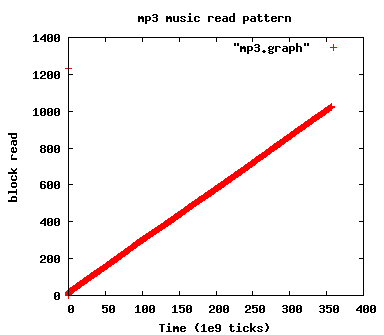
\includegraphics{filetype-mp3-graph.png}}
\caption{\small \bf Access pattern for an MP3 music file.}
\label{fig:filetype-mp3-graph}
\end{figure}

\begin{figure}[t!!]
\centering \resizebox{!}{2.8in}
{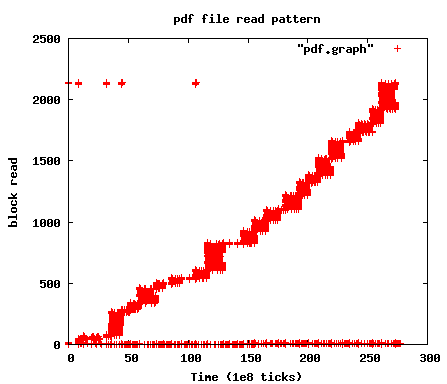
\includegraphics{filetype-pdf-adobe-graph.png}}
\caption{\small \bf Accesses for pdf using Acrobat reader.}
\label{fig:filetype-pdf-adobe-graph}
\end{figure}

\begin{figure}[t!!]
\centering \resizebox{!}{2.8in}
{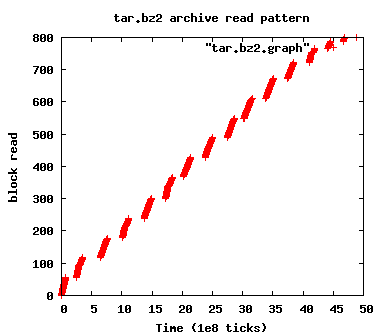
\includegraphics{filetype-bz2-graph.png}}
\caption{\small \bf Access pattern for a tar.bz2 archive.}
\label{fig:filetype-bz2-graph}
\end{figure}

\begin{figure}[t!!]
\centering \resizebox{!}{2.8in}
{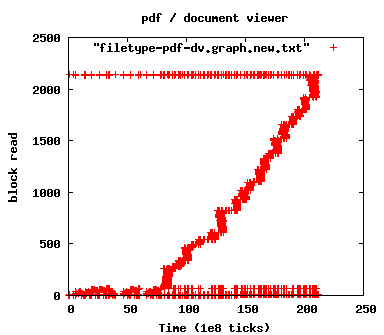
\includegraphics{filetype-pdf-dv-graph.png}}
\caption{\small \bf Access for pdf using Document Viewer.}
\label{fig:filetype-pdf-dv-graph}
\end{figure}

\begin{figure}[t!!]
\centering \resizebox{!}{2.8in}
{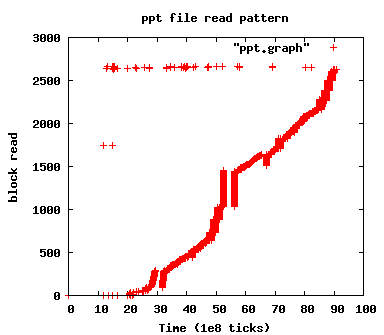
\includegraphics{filetype-ppt-graph.png}}
\caption{\small \bf Access pattern for a powerpoint presentation.}
\label{fig:filetype-ppt-graph}
\end{figure}

Figure~\ref{fig:filetype-pdf-adobe-graph} shows the access pattern for a PDF file using
Adobe reader. The access pattern is overall sequential but cut into chunks which are read repeatedly. This evidently gives us an opportunity to adjust prefetch window size close to the chunk size. There are also interleaved accesses to the end of the file, possibly due to accesses to font data, which would confuse the existing prefetching algorithm.

Figure~\ref{fig:filetype-pdf-dv-graph} shows the access pattern for the same PDF file
using the Gnome Document Viewer. Apart from the prolonged initial processing and an
increased number of reads to the head and tail of the file throughout the duration, the
access patterns are similar in their chunked nature. This builds upon our case for 
file-type based patterns in file accesses which lend themselves suitable to expoitation
by a prefetching algorithm.

Figure~\ref{fig:filetype-bz2-graph} shows the access pattern for a compressed archive(tar.bz2). The access pattern for
uncompressing the whole archive was purely sequential. This represents the case where
the existing prefetching algorithm works well.

Figure~\ref{fig:filetype-ppt-graph} shows the access pattern for a Powerpoint presentation(PPT). The access patterns
are similar to PDF, but the chunk sizes show a greater variance. This represents a 
case where rapid dynamic adaptation of prefetch window is required.

\subsection{Existing Implementation}

We analyzed the existing implementation of the prefetching algorithm in
the linux kernel. The algorithm, as we mentioned, does not account for
many of the possible factors, and therefore is quite simplistic.

Any file read starts off with a prefetch window size of 2 pages. If the kernel finds that
the file is being read sequentially, this window is doubled every time until either
the reads deviate from the sequential pattern or the hard limit of 32 on the prefetch
window size is reached. At any point, if the sequential read pattern stops and moves to a 
random pattern, the algorithm falls back to its initial state.

Quite evidently, one can see the insufficiencies with this approach. First off, particularly
with files like pdf, and ppt, where the read pattern is piecewise sequential, every 
jump causes the prefetching window to go back to the original value. Likewise, the 
hard static limit of 32 on the prefetch window size can be rather limiting on 
file types like video files which could benefit in terms of reduced jitter by 
having a large prefetch window. Also, the prefetch algorithm is currently implemented
independent of free space availability in the file-cache, thereby keeping open the
possibility that pages that were prefetched get evicted before they are actually used.

\section{Methodology}

This section describes the methodology we followed in devising our enhancements to
the prefetching algorithms. There are three parameters we identify about each
file that is being read. The first is the rate at which the file is being read.
This gives a measure of the value of prefetching a particular block into memory.
The second is the effect of cache-pressure. Through this we estimate the duration
for which a block lives in the cache. And finally we use file-type specific aspects
of the read pattern to optimize the prefetching algorithm, to the specific file
that is being accessed.

\subsection{Effect of read-rate}
The rate at which a file is being read gives an idea of the rate at which the 
application processes the file data, and therefore the estimated time at which
the next disk request is likely to happen. Of course, there are variations in 
read rate across different sections of the same file. To accommodate these variations
we determine long and short term averages of the read rates and compute our predicted
rate from these.

\subsection{Effect of cache-pressure}
With many reads happening simultaneously, it may happen that some of the data that
we prefetched may get evicted from the cache before it is actually used. This kind of 
a wasteful prefetching is a result of thrashing in the file-cache. Under such
circumstances, it would be advisable for the prefetching algorithm to backoff and prefetch
less. Towards this direction, we compute long and short term average lifetime of a 
page in the file-cache. We then use that to predict the expected cache-lifetime of the
pages we prefetch.

\subsection{Prefetch window calculation}
Once we have the estimated read rate of the file and the expected cache lifetime of
each prefetched page, we can compute the estimate of the ideal prefetch window based
on these factors. We then make use of this estimate to increase / decrease the 
prefetch window for the next readahead.

\subsection{Filetype specific policies}
In addition to the above two concerns, we note that different file-types have peculiarities
of their own in their access patterns. While simple examples would be files like mp3 and
avi which are read sequentially at a relatively constant rate; files like pdf etc tend to
have a piecewise sequential read pattern where a chunk of the file is read in and then read
over and over a few times before moving to the next chunk of the file. Also, there are
peculiarities like for eg: the first and last few pages of a pdf file are repeatedly read
throughout the entire application, which may confuse the existing prefetch algorithm. 
We decided that such peculiarities of access patterns can be used to provide hints to the
prefetching algorithm, but are best handled on a case by case basis.

\begin{figure*}[t!!]
\centering \resizebox{!}{3.7in}
{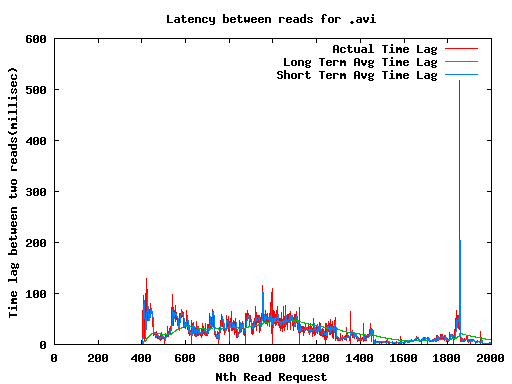
\includegraphics{avi-read-rate.png}}
\caption{\small \bf The instantaneous, short and long term read rates of an avi file.}
\label{fig:avi-read-rate}
\end{figure*}

\section{Implementation}

We implemented the enhanced prefetching algorithm on the linux kernel 2.6.27.5.
We employed RDTSC time-stamps within the prefetching and file-caching code to
determine the read rate of files and the cache-lifetime of pages. Likewise we modified
the open system-call handler to keep track of the file-type of the file for use
in the prefetching code. Each of these aspects of implementation are detailed below.

Since our code-changes are above the VFS layer, the behavior is expected to be
independent of the filesystem format.

\subsection{Measuring read-rates}

To determine the read rates, we instrumented the generic file read handler to insert
time-stamps and keep track of the previous block read and the time at which it was read.
With this information, instantaneous read rates are computed for each block and averaged
over a short as well as long interval to compute the short-term and long-term read rates.
The larger of these two values is then used as the current read-rate for the file.

Figure~\ref{fig:avi-read-rate} depicts the read rate computation. The instantaneous, short 
and long term time lag between reads as obtained from playing an avi video is graphed in 
the figure.

\subsection{Measuring cache-pressure}

Keeping track of cache pressure was the aspect of our implementation which we faced most
difficulty with. This primarily was due to the fact that the linux kernel cache replacement
policy is an approximate LRU and not a proper LRU. Thus the page evicted from the cache is
only probabilistically guaranteed to be the oldest, making it possible for newer pages to 
be evicted from the cache with non-zero probability.

However, we still were able to obtain an approximation for the lifetime of a page in the 
cache by using time-stamps to determine the duration between the last access and eviction
times of pages being evicted from the cache. We average this per-page value on a short term
and a long term basis to compute two cache-lifetime estimates. We then use the lower of the
two to adapt faster to rise in cache pressure while ramp up sluggishly when cache pressure
reduces.

For the limiting cases where the system has so far not seen any page eviction or the
system was left idle for long or the last page eviction happened considerably long ago,
we default to a pre-determined static value for the cache lifetime.

\subsection{Updating read-ahead window}

Finally we use the read rate and cache lifetime computed above to compute the ideal 
prefetch window for the next prefetch. We start reading with an initial prefetch 
window size, and double on each iteration until the prefetch window reaches
{\em EXP\_GROWTH\_LIMIT}. Thereafter, we increase the window size linearly by 
{\em GROWTH\_FACTOR}. This increasing phase is done subject to the condition that 
the current prefetch window lies below the ideal prefetch window size computed 
for this iteration. We have also placed an absolute upper bound of {\em WINDOW\_LIMIT}
on the size of the prefetch window as a worst case throttle.

If the current prefetch window size however is found to lie above the ideal for any
iteration, we immediately pull the current window size down to the ideal value to cut
back on cache pressure.

In the above process, we make use of the type of the file to adjust the algorithm 
to discount anomalous behavior expected in the file type (like last few pages read 
repeatedly in pdf files, as mentioned above).

\section{Evaluation}

We evaluated the modified prefetching algorithm on an ext3 partition on an
Intel Core2Duo 2 GHz. processor. We used a 160GB SATA disk @ 5400 RPM for 
all the evaluation runs.

\subsection{Workload}

Measuring and evaluating our file-type based corrections for sequentiality in the prefetching algorithm proved to be difficult.  Although we perceived the the delay in loading pdf files to have reduced, we do not have a reliably reproducable benchmark to cite as proof of our improvements.

For testing the impact of our algorithm under various read rates and cache pressure, we adopted the following strategy. We created processes that read a file from the disk at various read rates. With these, we measured the block read latency incurred in the kernel for each read request furnished by the application. In order to simulate cache pressure, we constrained the linux installation to a limited amount (256MB and 512MB) of RAM when performing our experiments and made sure that the file sizes we used exceeded the amount of free memory available in the system.

\subsection{Results}

\begin{figure}[t!!]
\centering \resizebox{!}{2.8in}
{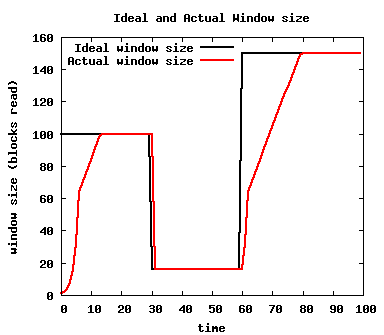
\includegraphics{window-size-pattern.png}}
\caption{\small \bf Plot of how our prefetch window size follows the ideal.}
\label{fig:window-size-pattern}
\end{figure}

Figure~\ref{fig:window-size-pattern} plots the ideal prefetch window size computed and how the actual window size used by our algorithm closely follows the same. When the window size is below the EXP\_GROWTH\_LIMIT (64 here) the increase is exponential. Thereafter the window size increases linearly until it matches the ideal window size. However, in the event that the computed ideal window size falls (due to extraneous facctors) we cut back on the actual window size to the same lower ideal window size to quickly respond to cache-pressure.

\begin{figure}[t!!]
\centering \resizebox{!}{2.8in}
{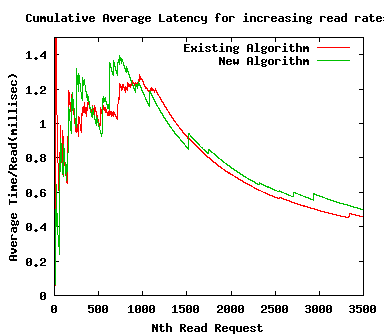
\includegraphics{file-read-rates.png}}
\caption{\small \bf Cumulative average latency for increasing read rates, without cache pressure.}
\label{fig:file-read-rates}
\end{figure}

Figure~\ref{fig:file-read-rates} shows the average time taken to service requests with increasing read rates on a single file. A program reads 4K bytes of data at a time from a file sequentially with the time lag between two requests dropping form 10000 to 20 microseconds over a period of 3500 reads. Initially both the algorithm have similar approaches and try to ramp up their read ahead window size. The existing algorithm stops after 32 pages, whereas we continue to increase our window size to WINDOW\_LIMIT (512here). But because of the way the LRU cache eviction works in linux, it kicks out some pages from our prefetched window causing intermediate spikes and hence we see an overall performance deterioation. We believe that fixing the LRU eviction algorithm will help us attain a more consistently better performance over the existing prefetching algorithm.

\begin{figure}[t!!]
\centering \resizebox{!}{2.8in}
{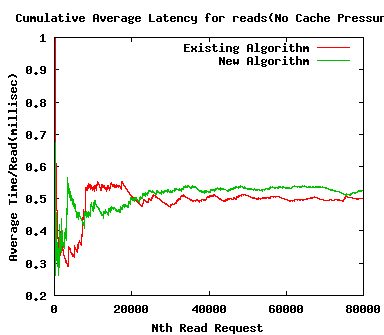
\includegraphics{file-copy-nocp-rates.png}}
\caption{\small \bf Cumulative average latency for constant rate reads in the absense of cache pressure.}
\label{fig:file-copy-nocp-rates}
\end{figure}

Figure~\ref{fig:file-copy-nocp-rates} is similar to figure~\ref{fig:file-read-rates} but with the read happening at a constant rate. Since there are not competing reads to the disk, the disk head rarely moves and hence the existing algorithm performs slightly better than our approach.

\begin{figure}[t!!]
\centering \resizebox{!}{2.8in}
{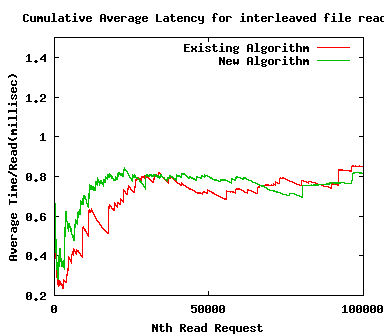
\includegraphics{interleave-rates-nocp.png}}
\caption{\small \bf Comparison of read latencies for interleaved reads in the absensce of cache pressure.}
\label{fig:interleave-rates-nocp}
\end{figure}

Figure~\ref{fig:interleave-rates-nocp} shows the interleaved read performance in the absence of cache pressure where our approach performs better on average because we prefetch more pages in one go and have overall reduced seek overheads. We got similar patterns on multiple runs and presume the spikes in the graph are caused by cache kicking out prefetched pages(which are always in the inactive list)

\begin{figure}[t!!]
\centering \resizebox{!}{2.8in}
{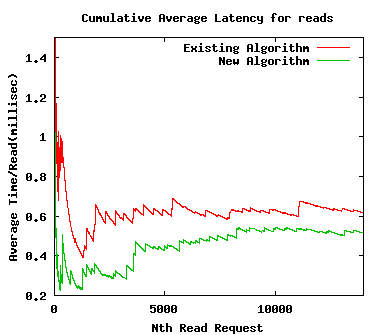
\includegraphics{cmp-avg-latency.png}}
\caption{\small \bf Comparison of read latencies with existing algorithm and
our modified algorithm under cache pressure.}
\label{fig:cmp-avg-latency}
\end{figure}

Figure~\ref{fig:cmp-avg-latency} depicts the read latencies when a single file is being read at a constant rate with cache presssure arising out of constrained memory limits. In this case we visibly outperform the existing linux prefetching algorithm by a factor of 16\%.

\begin{figure}[t!!]
\centering \resizebox{!}{2.8in}
{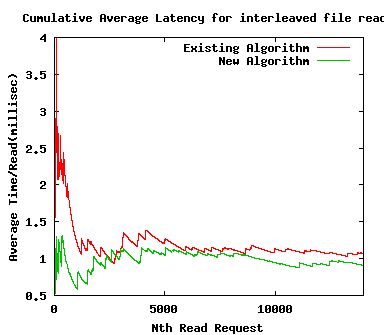
\includegraphics{cmp-avg-latency-2.png}}
\caption{\small \bf Comparison of interleaved read latencies with existing algorithm and
our modified algorithm under cache pressure.}
\label{fig:cmp-avg-latency-2}
\end{figure}

Figure~\ref{fig:cmp-avg-latency-2} depicts the read latencies when multiple files are being read in an interleaved fashion under a constrained cache. In this situation too, our algorithm outperforms the existing linux algorithm as we expected.

\section{Conclusion}

In conclusion, we find that adapting the prefetching algorithm to accommodate parameters like file-type, read rates and cache pressure improves the performance of file access under normal load patterns. However, on a lightly loaded system, this strategy may turn out to be counter productive because of the approximate implementation of the LRU cache eviction policy in linux. Yet, we believe that the tradeoff involved is reasonable since it essentially sums down to a slight increase in read latency under lighter loads as a price for an improvement in read latency under heavier system loads.

\section{Future Work}

As we mention earlier, one of the roadblocks we faced with our implementation
is the approximate nature of the linux LRU cache replacement algorithm. We're
working on figuring out ways to circumvent this and to introduce priorities for pages in the cache. With such a facility for eg., pages of an mp3 file which have already been read
once can be evicted from the cache in preference to pages from a pdf file.

We also plan to analyze read patterns for more file types and come up with an initial static read ahead window and ramp up size for them. Also currently our long term and short term averages are measured over somewhat arbitrary windows sizes. These may benefit from an empirical determination of the window over which the averages are best computed.

\begin{thebibliography}{99}

\bibitem[1]{1} Cao P, Edward W. Felten, Anna R and Y Kai Li.
	A study of integrated prefetching and caching strategies.
	In {\em Proceedings of the ACM SIGMETRICS}, 1995.
	
\bibitem[2]{2} Chuanpeng Li, Kai Shen, Athanasios E. Papathanasiou
	Competitive prefetching for concurrent sequential I/O.
	In {\em Proceedings of the 2nd ACM SIGOPS/EuroSys European Conference on Computer Systems}, 2007.

\bibitem[3]{3} James Griffioen.
	Reducing file system latency using a predictive approach.
	In {\em USENIX 94}, 1994.

\bibitem[4]{4} R. Hugo Patterson and Garth A. Gibson and Eka Ginting and Daniel Stodolsky and Jim Zelenka.
	Informed Prefetching and Caching.
	In {\em Proceedings of the Fifteenth ACM Symposium on Operating Systems Principles}, 1995.
	
\bibitem[5]{5} Fay W. Chang and Garth A. Gibson.
	Automatic I/O Hint Generation through Speculative Execution.
	In {\em Proceedings of the 3rd Symposium on Operating Systems Design and Implementation}, 1999.

\bibitem[6]{6} Shih, F.W.; Lee, T.-C.; Ong, S.
	A file-based adaptive prefetch caching design.
	In {\em Proceedings 1990 IEEE International Conference on Volume}, 1990.

\bibitem[7]{7} Ali R. Butt, Chris Gniady, Y. Charlie Hu
	The performance impact of kernel prefetching on buffer cache replacement algorithms.
	In {\em ACM SIGMETRICS Performance Evaluation Review Volume 33 , Issue 1}, 2005.

\bibitem[8]{8} Tulika Mitra, Chuan-Kai Yang, Tzi-cker Chiueh	.
	APPLICATION-SPECIFIC FILE PREFETCHING FOR MULTIMEDIA PROGRAMS.

\bibitem[9]{9}Phunchongharn, Phond Pornnapa, Supart Achalakul, Tiranee.
	File Type Classification for Adaptive Object File System.
	In {\em TENCON 2006 - IEEE Region 10 Conference}, 2006.

\bibitem[10]{10} K.-H. Kim, S.-H. Lim, and K.-H. Park.
	Adaptive Read-Ahead and Buffer Management for Multimedia Systems.
	In {\em Internet and Multimedia Systems and Applications}, 2004.
	
\bibitem[11]{11} Behdad Esfahbod.
	Preload � An Adaptive Prefetching Daemon.
	{\em Masters Thesis, Graduate Department of Computer Science. University of Toronto}, 2006.

\bibitem[12]{12} James Griffioen.
	Performance measurements of automatic prefetching.
	In {\em Proceedings of the ISCA International Conference on Parallel and Distributed Computing Systems}, 1995.

\bibitem[13]{13} Mark Palmer, Stanley B. Zdonik.
	Fido: A Cache That Learns To Fetch.
	In {\em Technical Report: CS-91-15, Brown University}, 1991.

%\bibitem[9]{9} Sung Hoon Baek, Kyu Ho Park.
%	Massive Stripe Cache And Prefetching for Massive File I/O.
%	In {\em ICCE 2007}, 2007.
	
\end{thebibliography}

\end{document}